\documentclass[12pt]{article}
% add some essential packages, some might not be used

\usepackage[T1]{fontenc}
\usepackage[utf8]{inputenc}
\usepackage[usenames,dvipsnames]{color}
\usepackage{natbib}
\usepackage{authblk}
\usepackage{ragged2e}
\usepackage{amsmath}
\usepackage[a4paper,margin=1in,bottom=1.0in]{geometry}
\usepackage{url}
\usepackage{array}
\usepackage{bbding}
\usepackage{amssymb}
\usepackage{graphicx}  % mini page function
\usepackage{adjustbox}
\usepackage{subcaption}
\usepackage{booktabs}
\usepackage{float}
\usepackage{appendix} % appendix package
\usepackage{hyperref}
\usepackage{url}
\usepackage[english]{babel}
\usepackage{adjustbox}
\usepackage{enumitem}
\usepackage{textgreek}
\usepackage{bibentry}
\nobibliography*
\usepackage{lipsum}


\usepackage{listings}
\usepackage{wasysym}
\usepackage{amsthm}
\usepackage{framed}
\usepackage{bm}
\usepackage{booktabs}  % package for table line
% \usepackage{amsrefs?}  % ams citation style package


\usepackage{rotating} % for the horizontal page table

\usepackage{tikz}
\usetikzlibrary{calc}
\usetikzlibrary{matrix}
\usetikzlibrary{positioning}
\usepackage{color}
\usepackage{setspace}
\usepackage{xcolor}

\usepackage{tcolorbox} % package for making colorful box

 \setlength{\parskip}{0.15cm} % change the paragraph spacing
\renewcommand\labelitemi{$\vcenter{\hbox{\tiny$\bullet$}}$} % set the bullet size as tiny

% \newcommand*\rot{\rotatebox{90}} % for rotate text

\usepackage{sectsty} %package for section size

\sectionfont{\fontsize{14}{12}\selectfont} % Change the section font size

\subsectionfont{\fontsize{13}{12}\selectfont}
\subsubsectionfont{\fontsize{12}{12}\selectfont}

\newcommand\numberthis{\addtocounter{equation}{1}\tag{\theequation}} % new command



\theoremstyle{definition}
\newtheorem{definition}[subsection]{Definition}
\newtheorem{axiom}[subsection]{Axiom}
\newtheorem{example}[subsubsection]{Example}
\newtheorem{theorem}[subsection]{Theorem}
\newtheorem{proposition}[subsection]{Proposition}
\newtheorem{lemma}[subsection]{Lemma}


\usepackage{courier}

% tikzsetting

\usetikzlibrary{shapes,decorations,arrows,calc,arrows.meta,fit,positioning}

\tikzset{
    -Latex,auto,node distance =1 cm and 1 cm,semithick,
    state/.style ={ellipse, draw, minimum width = 0.7 cm},
    point/.style = {circle, draw, inner sep=0.04cm,fill,node contents={}},
    bidirected/.style={Latex-Latex,dashed},
    el/.style = {inner sep=2pt, align=left, sloped}
}

\lstset{language=R}

\definecolor{mygreen}{rgb}{0,0.6,0}
\definecolor{mygray}{RGB}{145, 153, 165}
\definecolor{mymauve}{rgb}{0.58,0,0.82}

\lstset{
  backgroundcolor=\color{white},   % choose the background color; you must add \usepackage{color} or \usepackage{xcolor}; should come as last argument
  basicstyle=\footnotesize,        % the size of the fonts that are used for the code
  breakatwhitespace=false,         % sets if automatic breaks should only happen at whitespace
  breaklines=true,                 % sets automatic line breaking
  captionpos=b,                    % sets the caption-position to bottom
  commentstyle=\color{gray},    % comment style
  deletekeywords={...},            % if you want to delete keywords from the given language
  escapeinside={\%*}{*)},          % if you want to add LaTeX within your code
  extendedchars=true,              % lets you use non-ASCII characters; for 8-bits encodings only, does not work with UTF-8
  frame=single,	                   % adds a frame around the code
  keepspaces=true,                 % keeps spaces in text, useful for keeping indentation of code (possibly needs columns=flexible)
  keywordstyle=\color{RoyalBlue},       % keyword style
  language=R,                 % the language of the code
  morekeywords={*,...},            % if you want to add more keywords to the set
  numbers=left,                    % where to put the line-numbers; possible values are (none, left, right)
  numbersep=5pt,                   % how far the line-numbers are from the code
  numberstyle=\tiny\color{gray}, % the style that is used for the line-numbers
  rulecolor=\color{black},         % if not set, the frame-color may be changed on line-breaks within not-black text (e.g. comments (green here))
  showspaces=false,                % show spaces everywhere adding particular underscores; it overrides 'showstringspaces'
  showstringspaces=false,          % underline spaces within strings only
  showtabs=false,                  % show tabs within strings adding particular underscores
  stepnumber=2,                    % the step between two line-numbers. If it's 1, each line will be numbered
  stringstyle=\color{mymauve},     % string literal style
  tabsize=2,	                   % sets default tabsize to 2 spaces
  title=\lstname                   % show the filename of files included with \lstinputlisting; also try caption instead of title
}

\numberwithin{equation}{section}
\numberwithin{figure}{section}
\numberwithin{table}{section}


% Define colors
\definecolor{cmd}{HTML}{F7F7F9}
\DeclareMathOperator{\di}{d\!}

\newcommand{\pr}{$\mathbb{P}$}
\newcommand{\pre}{\mathbb{P}}

\begin{document}

\title{Non-stationary Time Series}
\author{Michael}
\date{}
\maketitle

\section{The Big Picture on Time Series}

I have to say it takes me a while to grasp the gist of \textit{time series}. Fortunately, I got the big picture, which can be the contour for doing empirical research in macroeconomics. For most students, the starting point of learning time series is the stationary process like AR(1) or MA(1). However, later I realised that lots of time series from real world are not stationary, which make researchers' life difficult and fun. So, what's the big picture of time series? Here we go: at this moment, it's about data-generating process for me.

Follow the idea by \cite{campbell1991pitfalls}, we assume that a time series $\{y_t\}$ is a realization of a deterministic trend and a stochastic component:
\begin{align}
  y_t = TD_t + z_t,
\end{align}
where $TD_t$ assigns a deterministic trend, which can be assumed to have the linear trend, $TD_t = \beta_1 + \beta_2 t$, and $z_t$ represents the stochastic compoment $\phi(L)z_t = \theta(L) \varepsilon_t$ with $\varepsilon_t \sim$i.i.d. Or expand it out, we have:
\begin{align*}
  y_t = \beta_0 + \beta_1 t + z_t; \ \ \ \ \ \phi(L)z_t = \theta(L) \varepsilon_t \ \ \varepsilon_t \sim i.i.d
\end{align*}

The intuition behind this assumption can be summarised by the following table:
\begin{table}[H]
  \centering
  \renewcommand{\arraystretch}{1.2}
  \title{Summary of data-generating process}
  \begin{tabular}{ccc}
    \hline
    \hline
    \multicolumn{2}{c}{\textbf{Deterministic Trend}} & \textbf{Stochastic Component} \\
    \hline
    Fixed effects & Trend & Stochastic pattern with random shocks \\
    \hline
    $\beta_1$ & $\beta_2 t$ & $\phi(L)z_t = \theta(L) \varepsilon_t$ \\
    \hline
    \multicolumn{2}{c}{Reflects Human Being's determination} & Law of nature (or unknown process) \\
    \hline
  \end{tabular}
\end{table}

For the deterministic trend, things are easy as we can predict it very well if they really follow a certain trend, which is highly unlikely in real data sets. It is common sense that everything is changing. Therefore, we care more about the stochastic part\footnote{or random part, think about normal distribution phenomena, then you will realise this part is the key.}.

Now, if all roots of the autoregressive polynomial lie outside the unit circle, then $\{y_t\}$ is stationary around a deterministic trend. In this case, one could remove the trend from the original series $\{y_t\}$ and fit an ARMA(p, q) to the residuals. In R programming, you can do it like this:
\begin{lstlisting}
  # Detrend the time series
  detrended <- residuals(lm(y ~ seq(along = y)))
  # fit ARMA model
  arma <- arima(detrend, ma=..., ar=...,)
\end{lstlisting}

The \textit{trend-stationary} model is also called the integrated model of order zero or $I(0)$. But, what if some roots lie on the unit circle\footnote{we don't consider the cases that roots are inside the unit circle as $y_t$ will explore in this case.}? If it happens, things become tricky and that's why I am writing this notes now. For the unit root situation, $\Delta z_t = (1-L) z_t$ is stationary around a constant mean, the series $\{y_t\}$ is \textit{difference-stationary} because one has to apply the first difference filter with respect to time to obtain a stationary process. This process can be analyzed with \textit{autoregressive integrated moving average} (ARIMA)(p, d, q), where d refers to the order of intergration.

\textbf{Take away}: by decomposing time series $\{y_t\}$, we realise that stochastic part is the key, and unit root situation is the aiming ring.

Before we moving to the next section, let's state the distinction between a trend- and a difference-stationary process by giving the following two processes:
\begin{align}
  y_t  & = y_{t-1} + \mu = y_0 + \mu t \\
  y_t & = y_{t-1} + \varepsilon_t = y_0 + \sum_{s=1}^t \varepsilon_s
\end{align}

\section{Unit Root Processes}

As we have said that unit root processes are so important, it's worth to devote ourselves to this topic. Let's review the data-generating process:
\begin{align}
  y_t & = y_0 + \mu t + z_t \\
      & = y_0 + \mu t + (\phi(L) z_t = \theta(L) \varepsilon_t)
\end{align}
Now, let's decompose the stochastic component $z_t$ into a cyclical component $c_t$ and a stochastic trend $TS_t$. It is assumed that \textit{cyclical component} $c_t$ is a mean-stationary process. Then, equation (2.1) can be rewritten as
\begin{align}
  y_t = y_0 + \mu t + c_t + TS_t
\end{align}

Equation (2.3) will be the \textbf{key function} for almost all our analysis in this document. Now, let's list all situations for $y_t$ in equation (2.3):
\begin{itemize}
  \item If $y_t$ is trend stationary, then the stochastic trend ($TS_t$) is zero. Then, $y_t$ can be modeled by ARMA(p, q).
  \item If $y_t$ is difference stationary, then the autoregressive polynomial contains a unit root that can be factored out by doing the difference, $\phi(L) = (1- L)\phi^{*}(L)$. After doing the difference, we get $\Delta z_t$ which can be modeled as the moving average process.
\end{itemize}

Now, if we represent $z_t = TS_t + c_t = \psi(1) S_t + \psi^{*}(L) \varepsilon_t$, where $\psi(1)$ is the sum of moving average coefficients and $S_t$ is the sume of the past and present of random shocks $\sum_{s=1}^t \varepsilon_s$, and $\psi^{*}(L)$ is the polynomial coefficients. The full equation is\footnote{Check equation (1.3), to see what's going on.}:
\begin{align}
  z_t = c_t + TS_t = \psi(1) \sum_{s=1}^t \varepsilon_s + \frac{\psi(L) - \psi(1)}{(1 - L)} \varepsilon_t
\end{align}

Final step, substitute (2.4) into (2.3) to get:
\begin{align}
  y_t & = y_0 + \mu t + TS_t + c_t \\
      & = y_0 + \mu t + \psi(1) \sum_{s=1}^t \varepsilon_s + \frac{\psi(L) - \psi(1)}{(1 - L)} \varepsilon_t
\end{align}

I am sorry to reclaim that equation (2.6) will be the \textbf{key function} for almost all our analysis of time series data. The intuition and summary on (2.6) is given in Figure 2.2.
\begin{figure}[H]
  \centering
  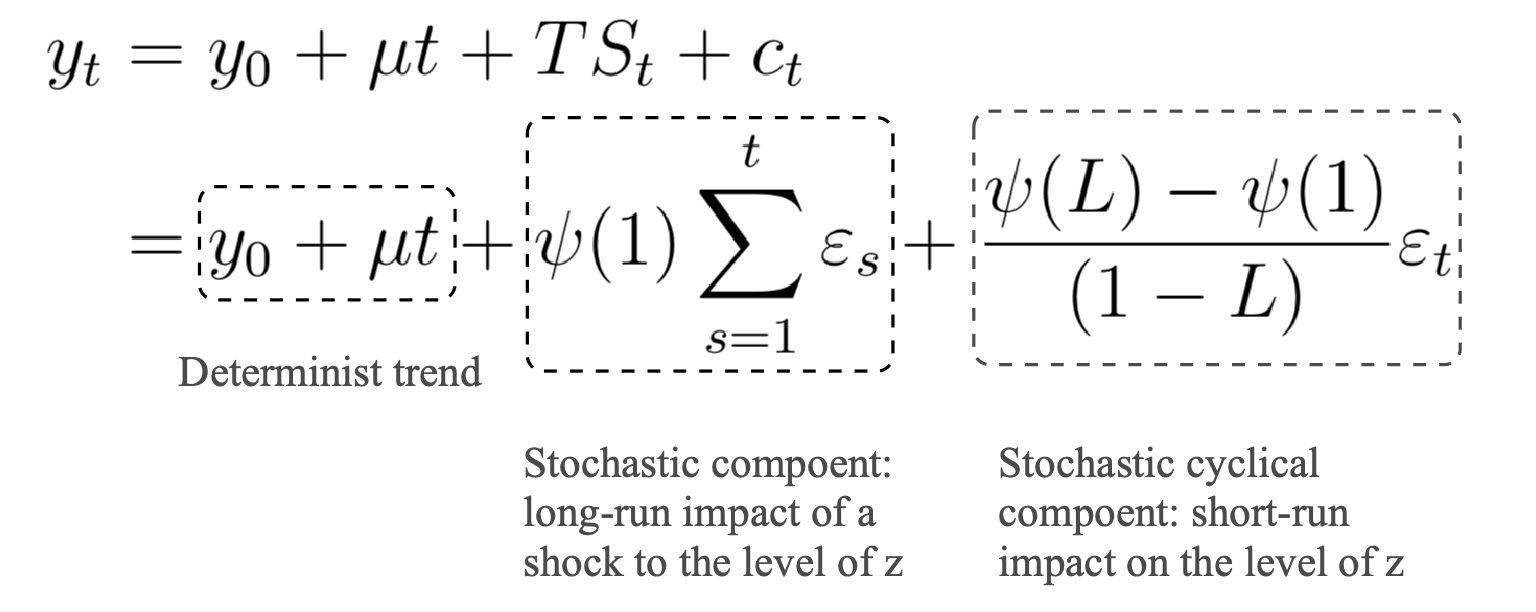
\includegraphics[width=0.69\textwidth]{ydecom}
  \caption{Intuition on $y_t$ decomposition}
\end{figure}










\newpage
\bibliography{/Users/Michael/Documents/DSGE/dsge.bib}
\bibliographystyle{apalike}
\end{document}
